\documentclass[compress]{beamer}

\usetheme{Hamburg}

\usepackage[utf8]{inputenc}
\usepackage{units}

\usepackage[absolute,overlay]{textpos}
  \setlength{\TPHorizModule}{1mm}
  \setlength{\TPVertModule}{1mm}

\title{IVC - Zwischenpräsentation}
\author{Thorben Harms, Felix Ortmann \& Kai Hildebrandt}
\institute{Fachbereich Informatik\\Fakultät für Mathematik, Informatik und Naturwissenschaften\\Universität Hamburg}
\date{18.12.2013}

\titlegraphic{
\includegraphics[width=0.5\textwidth]{logo}}


\begin{document}

\begin{frame}
	\titlepage
\end{frame}

\begin{frame}
	\frametitle{Gliederung}

	\tableofcontents[hidesubsections]
\end{frame}

\section{Idee}

\begin{frame}
	\frametitle{Idee}

	\begin{itemize}
	  \item<+-> Ein Blatt Papier ist zu sehen, auf das ein Strichmännchen gemalt ist.
	  \item<+-> Eine Windhose saugt das Strichmännchen ,,aus dem Papier" in eine dreidimensionale Welt.
	  \item<+-> Dort passieren Dinge... Das ist bewusst offen gehalten ;)
	  \item<+-> Das Strichmännchen fällt zurück ,,in das Papier" und liegt anders dort, als zu Beginn.
	  \item<+-> Zusammen mit dem Strichmännchen ist ein Würfel mit auf das Blatt Papier gefallen, der allerdings nicht ,,in das Papier" übergeht, sondern materialisiert auf dem Tisch liegen bleibt.
	\end{itemize}
\end{frame}

\section{Aktueller Stand}

\begin{frame}
	\frametitle{Aktueller Stand}
	\vspace{0.5cm}
	verschiedene Objekte erstellt:	
	\begin{itemize}
	  \item Strichmännchen
	  \item Windhose
	  \item Würfel
	  \item Tisch
	  \item etc.
	\end{itemize}
	
	
	\begin{textblock}{100}(80,15)
	  
\includegraphics[width=3cm]{pics/maenchen.png}
	\end{textblock}
	\vspace{1.5cm}
	\begin{figure}
		\begin{center}
			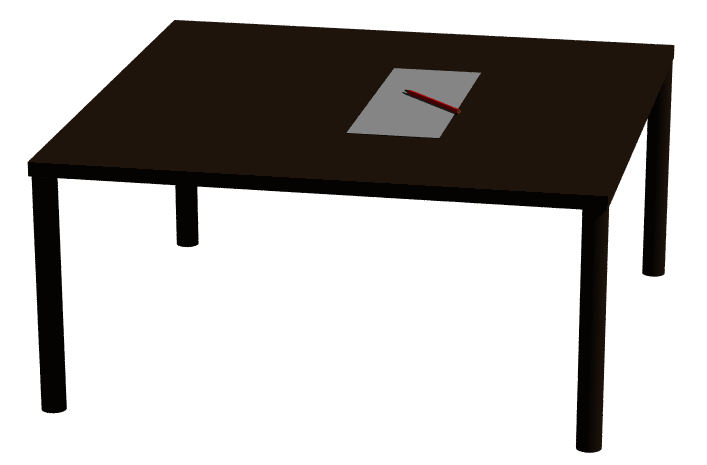
\includegraphics[width=0.3\textwidth]{pics/table.png}
			
\includegraphics[width=0.2\textwidth]{pics/tornado3.png}
			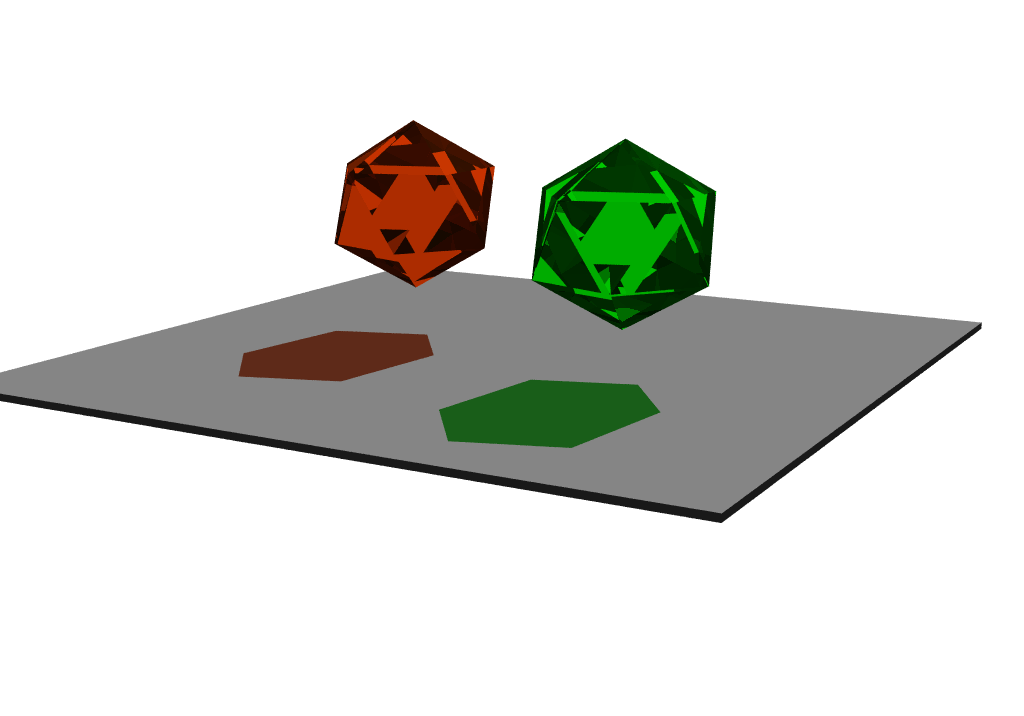
\includegraphics[width=0.2\textwidth]{pics/rotating_dices08.png}
			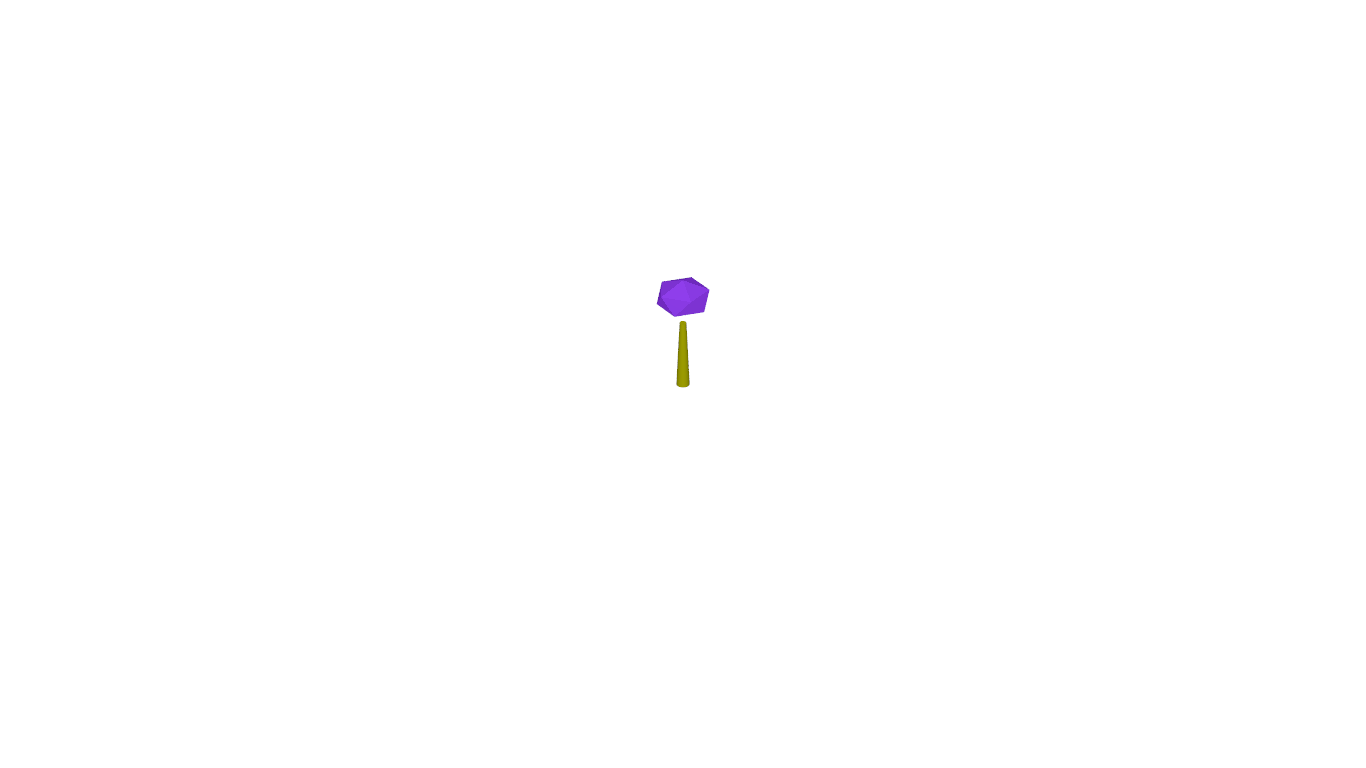
\includegraphics[width=0.1\textwidth]{pics/solo_stick.png}
			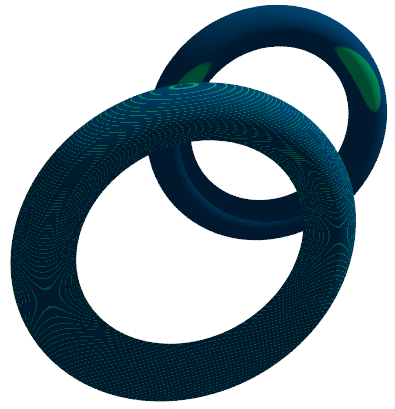
\includegraphics[width=0.2\textwidth]{pics/texturemapping.png}
		\end{center}
	\end{figure}

\end{frame}

\end{document}
